% Standalone vector figure extracted from manuscript.tex.
% Rebuild all figures from the project root: bash tkz/build.sh
\documentclass[tikz,border=2pt,class=IEEEtran]{standalone}
\usepackage{amsmath,amssymb,amsfonts}
\usepackage{xcolor}
\usetikzlibrary{positioning,arrows.meta,calc,backgrounds}

% Match the manuscript's IEEE Access text and math font settings.
\renewcommand{\textbf}[1]{{\fontseries{b}\selectfont #1}}
\renewcommand{\textit}[1]{{\itshape #1}}
\makeatletter
\AtBeginDocument{%
  \fontencoding{T1}\rmfamily\fontseries{m}\fontsize{10}{12}\selectfont
  \gdef\operator@encoding{T1}%
  \gdef\encodingdefault{T1}}
\makeatother

% ---- shared palette for review figures ----
\definecolor{cVLA}{HTML}{34618E}   % VLA lane / policy blue
\definecolor{cWM}{HTML}{9E4A3F}    % world-model lane
\definecolor{cCONV}{HTML}{5E4B8B}  % convergence purple
\definecolor{cGood}{HTML}{3A7D44}  % verified green
\definecolor{cWarn}{HTML}{B07A2A}  % caution amber
\definecolor{cPale}{HTML}{F2F0EA}  % pale panel fill
\tikzset{
  fnode/.style={draw=black!55, fill=white, rounded corners=1.5pt,
                inner sep=2.5pt, align=center, font=\fontsize{8}{9.5}\selectfont},
  flane/.style={draw=none, rounded corners=2pt, inner sep=3pt,
                align=center, font=\fontsize{8}{9.5}\selectfont\bfseries, text=white},
  farr/.style={-{Stealth[length=2mm]}, thick, black!60},
}


\newcommand{\figfont}{\fontsize{8}{9.5}\selectfont}

\begin{document}

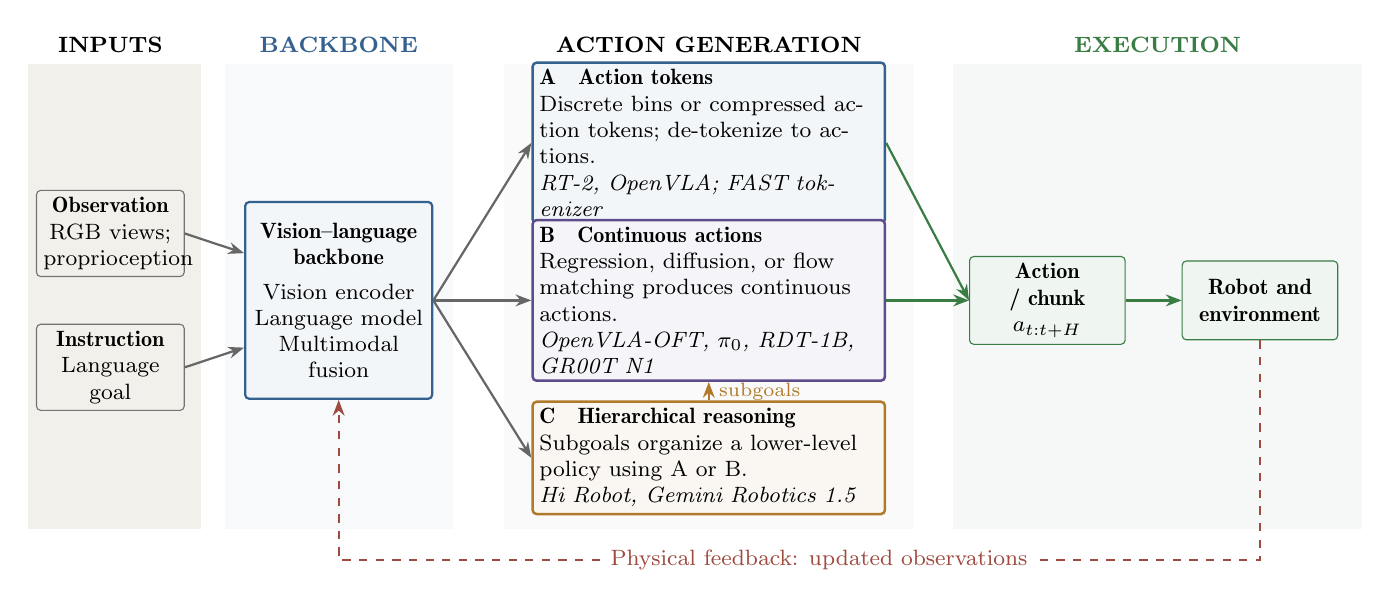
\begin{tikzpicture}[font=\figfont]
\tikzset{box/.style={fnode,minimum height=10mm},
 dec/.style 2 args={fnode,draw=#1,line width=.9pt,fill=#1!6,text width=#2,align=left},
 a/.style={farr,line width=.8pt}}
\begin{scope}[on background layer]
\fill[cPale] (-1.05,-2.9) rectangle (1.15,3.0);
\fill[cVLA!4] (1.45,-2.9) rectangle (4.35,3.0);
\fill[black!2] (5,-2.9) rectangle (10.2,3.0);
\fill[cGood!5] (10.7,-2.9) rectangle (15.9,3.0);
\end{scope}
\node[font=\figfont\bfseries] at (0,3.25) {INPUTS};
\node[font=\figfont\bfseries,cVLA] at (2.9,3.25) {BACKBONE};
\node[font=\figfont\bfseries] at (7.6,3.25) {ACTION GENERATION};
\node[font=\figfont\bfseries,cGood] at (13.3,3.25) {EXECUTION};
\node[box,fill=cPale,text width=17mm] (obs) at (0,.85) {\textbf{Observation}\\RGB views;\\proprioception};
\node[box,fill=cPale,text width=17mm] (lang) at (0,-.85) {\textbf{Instruction}\\Language goal};
\node[box,draw=cVLA,thick,fill=cVLA!6,text width=22mm,minimum height=25mm] (core) at (2.9,0) {\textbf{Vision--language backbone}\\[3pt]Vision encoder\\Language model\\Multimodal fusion};
\draw[a] (obs.east)--([yshift=6mm]core.west);
\draw[a] (lang.east)--([yshift=-6mm]core.west);
\node[dec={cVLA}{43mm}] (a) at (7.6,2.0) {\textbf{A\quad Action tokens}\\Discrete bins or compressed action tokens; de-tokenize to actions.\\\textit{RT-2, OpenVLA; FAST tokenizer}};
\node[dec={cCONV}{43mm}] (b) at (7.6,0) {\textbf{B\quad Continuous actions}\\Regression, diffusion, or flow matching produces continuous actions.\\\textit{OpenVLA-OFT, $\pi_0$, RDT-1B, GR00T~N1}};
\node[dec={cWarn}{43mm}] (c) at (7.6,-2.0) {\textbf{C\quad Hierarchical reasoning}\\Subgoals organize a lower-level policy using A or B.\\\textit{Hi Robot, Gemini Robotics 1.5}};
\draw[a] (core.east)--(a.west);
\draw[a] (core.east)--(b.west);
\draw[a] (core.east)--(c.west);
\draw[a,cWarn,dashed] (c.north)-- node[right,font=\fontsize{7.5}{9}\selectfont]{subgoals} (b.south);
\node[box,draw=cGood,fill=cGood!8,text width=18mm] (act) at (11.9,0) {\textbf{Action / chunk}\\$a_{t:t+H}$};
\node[box,draw=cGood,fill=cGood!8,text width=18mm] (env) at (14.6,0) {\textbf{Robot and environment}};
\draw[a,cGood] (a.east)--(act.west);
\draw[a,cGood] (b.east)--(act.west);
\draw[a,cGood] (act)--(env);
\draw[a,cWM,dashed] (env.south)--(14.6,-3.3)--(2.9,-3.3)--(core.south);
\node[fill=white,inner sep=2pt,text=cWM] at (9,-3.3) {Physical feedback: updated observations};
\end{tikzpicture}
\end{document}
